\chapter{Visão Geral de Métodos de Otimização}

Visão geral de métodos mais avançados que não foram vistos durante o curso

\section{Métodos exatos}

\begin{itemize}
	\item Programação dinâmica
	\item Programação por restrições (Constraint programming) $\rightarrow$ Baseado em apresentar as restrições que a solução tem que ter. Não é necessariamente linear. Existem resolvedores para isso.
\end{itemize}

\subsection{Programação dinâmica}

Resolver um problema dividindo a entrada em menores do mesmo tipo. $\rightarrow$ Divisão e conquista. Mas o que difere é que os resultados dos subproblemas são armazenados para não ter que recomputar.

\begin{itemize}
	\item O problema tem que ter uma subestrutura ótima. $\rightarrow$ A solução ótima é composta de soluções ótimas dos subproblemas
	\item Os problemas tem que compartilhar subproblemas (para que valha a pena armazenar os resultados).
\end{itemize}

\subsubsection{Fibonacci}

\begin{algorithm}
	\SetAlgoLined
	\SetKwFunction{FibonacciUm}{FibonacciRec}
	\Fn{\FibonacciUm{n}}{
		\Se{$n \leq 2$}{
			\Retorna{1}
		}
		\Retorna{\FibonacciUm{n-1} $+$ \FibonacciUm{n-2}}
	}
\end{algorithm}

O problema com esse algoritmo recursivo básico, é que muitos subproblemas são constantemente recalculados. $\rightarrow$ O método fica ineficiente

Para solucionar esse problema, podemos usar a memória para armazenar os valores já calculados em uma tabela.

\begin{algorithm}
	\SetAlgoLined
	\SetKwFunction{FibonacciDois}{FibonacciPD}
	\Fn{\FibonacciDois{n}}{
		Seja $F$ um vetor de tamanho $n$\;
		$F[1] \gets F[2] \gets 1$\;
		\Para{$i \gets 3$ até $n$}{
			$F[i] \gets F[i-1] + F[i-2]$\;
		}
		\Retorna{$F[n]$}
	}
\end{algorithm}

A tabela nesse caso é unidimensional. Mas pode ter várias outras dimensões, depende do número de índices que variam no problema. A ideia básica é, porém, preencher a tabela conforme vai resolvendo os subproblemas.

\subsubsection{Problema da Mochila Binária}

Seja $S* \subseteq \left\{ 1, 2, \dots, n\right\}$ uma solução ótima para $I = (\left\{ 1, 2, \dots, n\right\}, v, w, W)$. Temos duas possibilidades:

\begin{itemize}
	\item $n \notin S*$, caso em que $S*$ é solução ótima de $(\left\{ 1, 2, \dots, n-1\right\}, v, w, W) \rightarrow$ O item $n$ não está na mochila, então a solução ótima é a mesma do caso em que ele não estivesse lá para ser escolhido, mantendo o peso e os valores.
	\item $n \in S*$, caso em que $S* \setminus \left\{ n\right\}$ é solução ótima de $(\left\{ 1, 2, \dots, n-1\right\}, v, w, W-w_n) \rightarrow$ Como $n$ está na mochila, podemos encontrar uma solução ótima com os outros itens e temos também que retirar a capacidade dele da mochila.
\end{itemize}

Sendo $V_{i, T}$ o custo de uma solução ótima que escolhe itens no subconjunto $\left\{ 1, 2, \dots, i\right\}$ para preencher uma mochila de capacitade $T$, temos:

\[
	V_{i,T} =
	\begin{cases}
		\max\left\{ V_{i-1, T}, V_{i-1, T-w_i} + v_i\right\} & \quad \text{se } w_i \leq T \\
		V_{i-1, T}                                           & \quad \text{se } w_i > T
	\end{cases}
\]

Temos que verificar se o item $i$ cabe na mochila ($w_i \leq T$). Se couber, verificamos se vale a pena colocá-lo ou não ($\max$).

\begin{example}
	$w_1 = 1, v_1 = 1$

	$w_2 = 3, v_2 = 2$

	$w_3 = 2, v_3 = 1$

	$w_4 = 1, v_4 = 2$

	$w_5 = 4, v_5 = 6$

	Capacidade da mochila: $W = 4$

	Caso base: a mochila não tem capacidade, não podemos considerar nenhum item. Então o valor vai ser necessariamente $0$. Também tem o caso em que não há nenhum item para ser verificado ($i = 0$), como não podemos pegar nenhum item, o valor também é $0$.

	\begin{center}
		\begin{tabular}{c|c|c|c|c|c|}
			\cline{2-6}
			5                                              & 0                     &                       &                       &                       &                       \\ \cline{2-6}
			4                                              & 0                     &                       &                       &                       &                       \\ \cline{2-6}
			3                                              & 0                     &                       &                       &                       &                       \\ \cline{2-6}
			2                                              & 0                     &                       &                       &                       &                       \\ \cline{2-6}
			1                                              & 0                     &                       &                       &                       &                       \\ \cline{2-6}
			0                                              & 0                     & 0                     & 0                     & 0                     & 0                     \\ \cline{2-6}
			\multicolumn{1}{c}{\diagbox[dir=NE]{$i$}{$T$}} & \multicolumn{1}{c}{0} & \multicolumn{1}{c}{1} & \multicolumn{1}{c}{2} & \multicolumn{1}{c}{3} & \multicolumn{1}{c}{4}
		\end{tabular}
	\end{center}

	Começamos incrementando o $i$ e o $T$. Por exemplo, no caso em que  $i=1, T=1$, temos que o item $i$ cabe na mochila ($w_i \leq T$). Então, calculamos os valores da expressão de maximização. Preenchendo a linha toda:

	\begin{center}
		\begin{tabular}{c|c|c|c|c|c|}
			\cline{2-6}
			5                                              & 0                     &                       &                       &                       &                       \\ \cline{2-6}
			4                                              & 0                     &                       &                       &                       &                       \\ \cline{2-6}
			3                                              & 0                     &                       &                       &                       &                       \\ \cline{2-6}
			2                                              & 0                     &                       &                       &                       &                       \\ \cline{2-6}
			1                                              & 0                     & 1                     & 1                     & 1                     & 1                     \\ \cline{2-6}
			0                                              & 0                     & 0                     & 0                     & 0                     & 0                     \\ \cline{2-6}
			\multicolumn{1}{c}{\diagbox[dir=NE]{$i$}{$T$}} & \multicolumn{1}{c}{0} & \multicolumn{1}{c}{1} & \multicolumn{1}{c}{2} & \multicolumn{1}{c}{3} & \multicolumn{1}{c}{4}
		\end{tabular}
	\end{center}

	Preenchendo a linha em que consideramos o item 2, temos os casos em que ele não cabe na mochila e simplesmente pegamos os valores anteriores (abaixo, em que pegamos só o item 1).

	\begin{center}
		\begin{tabular}{c|c|c|c|c|c|}
			\cline{2-6}
			5                                              & 0                     &                       &                       &                       &                       \\ \cline{2-6}
			4                                              & 0                     &                       &                       &                       &                       \\ \cline{2-6}
			3                                              & 0                     &                       &                       &                       &                       \\ \cline{2-6}
			2                                              & 0                     & 1                     & 1                     &                       &                       \\ \cline{2-6}
			1                                              & 0                     & 1                     & 1                     & 1                     & 1                     \\ \cline{2-6}
			0                                              & 0                     & 0                     & 0                     & 0                     & 0                     \\ \cline{2-6}
			\multicolumn{1}{c}{\diagbox[dir=NE]{$i$}{$T$}} & \multicolumn{1}{c}{0} & \multicolumn{1}{c}{1} & \multicolumn{1}{c}{2} & \multicolumn{1}{c}{3} & \multicolumn{1}{c}{4}
		\end{tabular}
	\end{center}

	Mas agora temos o caso em que $T=3$, ou seja, o item 2 cabe na mochila. Nesse caso, vemos se vale a pena pegá-lo ou não. O caso de não pegá-lo, temos o valor $V_{i-1, T} = 1$. O caso de pegá-lo, temos $V_{i-1,  T-w_i}+v_i = V_{1, 0} + 2 = 2$. Então vale mais a pena pegar o item 2.

	Já no caso em que $T=4$, temos que $V_{i-1, T-w_i}+v_i = V_{1, 1} + 2$, ou seja, ainda há espaço livre de valor 1, em que cabe o item 1, resultando então no valor final de 3.

	\begin{center}
		\begin{tabular}{c|c|c|c|c|c|}
			\cline{2-6}
			5                                              & 0                     &                       &                       &                       &                       \\ \cline{2-6}
			4                                              & 0                     &                       &                       &                       &                       \\ \cline{2-6}
			3                                              & 0                     &                       &                       &                       &                       \\ \cline{2-6}
			2                                              & 0                     & 1                     & 1                     & 2                     & 3                     \\ \cline{2-6}
			1                                              & 0                     & 1                     & 1                     & 1                     & 1                     \\ \cline{2-6}
			0                                              & 0                     & 0                     & 0                     & 0                     & 0                     \\ \cline{2-6}
			\multicolumn{1}{c}{\diagbox[dir=NE]{$i$}{$T$}} & \multicolumn{1}{c}{0} & \multicolumn{1}{c}{1} & \multicolumn{1}{c}{2} & \multicolumn{1}{c}{3} & \multicolumn{1}{c}{4}
		\end{tabular}
	\end{center}

	Continuando, incluindo os outros itens:

	\begin{center}
		\begin{tabular}{c|c|c|c|c|c|}
			\cline{2-6}
			5                                              & 0                     & 2                     & 3                     & 3                     & 6                     \\ \cline{2-6}
			4                                              & 0                     & 2                     & 3                     & 3                     & 4                     \\ \cline{2-6}
			3                                              & 0                     & 1                     & 1                     & 2                     & 3                     \\ \cline{2-6}
			2                                              & 0                     & 1                     & 1                     & 2                     & 3                     \\ \cline{2-6}
			1                                              & 0                     & 1                     & 1                     & 1                     & 1                     \\ \cline{2-6}
			0                                              & 0                     & 0                     & 0                     & 0                     & 0                     \\ \cline{2-6}
			\multicolumn{1}{c}{\diagbox[dir=NE]{$i$}{$T$}} & \multicolumn{1}{c}{0} & \multicolumn{1}{c}{1} & \multicolumn{1}{c}{2} & \multicolumn{1}{c}{3} & \multicolumn{1}{c}{4}
		\end{tabular}
	\end{center}
\end{example}

A solução final (valor final da mochila) está armazenada na última posição, em que $i=n$ e $T=W$.

\begin{algorithm}
	\SetAlgoLined
	\SetKwFunction{MochilaPD}{MochilaPD}
	\Fn{\MochilaPD{$n, w, v, W$}}{
		seja $M$ uma matriz de tamanho $(n+1) \times (W+1)$\;
		\Para{$T \gets 0$ até $W$}{
			$M[0][T] \gets 0$\;
		}
		\Para{$i \gets 1$ até $n$}{
			\Para{$T \gets 0$ até $W$}{
				\eSe{$w_i > T$}{
					$M[i][T] \gets M[i-1][T]$\;
				}{
					$M[i][T] \gets \max\left\{ m[i-1][T], M[i-1][T-w_i]+v_i\right\}$\;
				}
			}
		}
		\Retorna{M[n][W]}
	}
\end{algorithm}

\vfill

\section{Algoritmos de aproximação}

Outra abordagem para lidar com problemas de otimização combinatória, são os algoritmos de aproximação. São um ``caminho do meio'' entre métodos exatos e heurísticas.

Algoritmos são algoritmos que executam em tempo polinomial, sem garantir que a solução seja ótima. Mas podemos garantir que a solução está dentro de um intervalo com relação ao custo da solução ótima.

Seja A um algoritmo polinomial para um problema de minimização, $A(I)$ o custo da solução de $A$ para a entrada $I$ e $\mathrm{OPT}(I)$ o custo da solução ótima.

A é uma $\alpha$-aproximação se, para toda instância $I$,

\[
	A(I) \leq \alpha \cdot \mathrm{OPT}(I) \rightarrow \text{Razão de aproximação}
\]

Se o problema for de maximização, invertemos a desigualdade.

\[
	A(I) \geq \alpha\cdot \mathrm{OPT}(I)
\]

\subsection{Problema da Mochila Binária}

\begin{algorithm}
	\SetAlgoLined
	\SetKwFunction{MochilaAprox}{MochilaAprox}
	\Fn{\MochilaAprox{$n, w, v, W$}}{
		Ordene e renomeie os itens para que $\frac{v_1}{w_1}\geq\frac{v_2}{w_2}\geq\dots\geq\frac{v_n}{w_n}$\;
		\tcc{Cabe até o item $q$, mas o $q+1$ não cabe mais}
		Seja $q$ um inteiro tal que $\sum_{i=1}^qw_i\leq W$ e $\sum_{i=1}^{q+1}w_i>W$\;
		\Retorna{$\max\left\{ v_1 + v_2 + \dots + v_q, v_{q+1}\right\}$}
	}
\end{algorithm}

Temos que o valor máximo entre dois valores é claramente maior que a média da soma dos valores: $\max\left\{ a, b\right\} \geq \frac{a+b}{2}$. Assim, temos:

\begin{align*}
	\text{\lstinline{MochilaAprox}}(I) &= \max\left\{ v_1 + v_2 + \dots + v_q, v_{q+1}\right\} \\
	  & \geq \frac{1}{2}\left( v_1 + \dots + v_q + v_{q+1} \right) \\
	  & \geq \frac{1}{2}\mathrm{OPT}_{\mathrm{frac}}(I)            \\
	  & \geq \frac{1}{2}\mathrm{OPT}(I)
\end{align*}

Sabemos que $(v_1+\dots+v_q+v_{q+1})$ não cabe na mochila e que vai ser maior ou igual que a solução ótima da mochila fracionária, já que ordenamos os itens seguindo sua densidade e isso nos dá a solução ótima da mochila fracionária. Também sabemos que a solução ótima da mochila fracionária sempre será maior ou igual à solução da mochila inteira, pois ela vem da sua relaxação.

Com isso, temos que esse algoritmo é uma $\frac{1}{2}$-aproximação.

\subsection{Problema do Escalonamento}

\begin{algorithm}
	\SetAlgoLined
	\SetKwFunction{EscalonaAprox}{EscalonaAprox}
	\Fn{\EscalonaAprox{$n, t, m$}}{
	\lPara{$j \gets 1$ até $m$}{$M_j \gets \emptyset$}
	\Para{$i \gets 1$ até $n$}{
	Seja $j$ uma máquina em que $\sum_{i' \in M_j}t_{i'}$ é mínimo\;
	$M_j \gets M_j \bigcup \left\{ i\right\}$\;
	}
	\Retorna{$\max_{j=1,\dots,m}\sum_{i \in M_j}t_i$}
	}
\end{algorithm}

O algoritmo é o mesmo algoritmo guloso usado na \hyperref[chp:semana2]{Semana 2}. Mas ele é de aproximação também porque temos uma garantia de qualidade da solução.

Seja $j$ a máquina que define o \textit{makespan} e seja $k$ a última tarefa que foi alocada a essa máquina. No momento em que a tarefa $k$ foi colocada na máquina $j$, essa máquina era a máquina menos carregada (devido ao critério guloso do algoritmo), ou seja, naquele momento $M_j$ tinha carga menor ou igual a qualquer outra máquina.

Seja $l(j)=\sum_{i \in M_j}t_i$ a carga da máquina $j$. Qualquer máquina $j'$ tem carga $l(j')\geq l(j)-t_k$ (antes de colocar o item $k$, a máquina $j$ é a de menor carga). Então

\[
	(l(j)-t_k) \cdot m \leq \sum_{j'=i}^ml(j') = \sum_{i=1}^nt_i
\]

Temos que esse valor é sempre menor que o valor da carga de todas as máquinas, que no fim é apenas a carga de todas as tarefas.

Dividindo por $m$:

\[
	l(j)-t_k \leq \frac{\sum_{i=1}^nt_i}{m} = \mathrm{OPT}_{\mathrm{frac}}(I) \leq \mathrm{OPT}(I)
\]

Temos que a solução ótima do escalonamento fracionário é simplesmente dividir igualmente os tempos das tarefas sobre todas as máquinas.

\[
	l(j)-t_k \leq \mathrm{OPT}(I)
\]

Assim

\begin{align*}
	\text{\lstinline{EscalonaAprox}}(I) & = l(j)                                 \\
	                                    & = (l(j)-t_k)+t_k                       \\
	                                    & \leq \mathrm{OPT}(I) + t_k             \\
	                                    & \leq \mathrm{OPT}(I) + \mathrm{OPT}(I) \\
	                                    & =2 \mathrm{OPT}(I)
\end{align*}

Assim, o algoritmo é uma 2-aproximação.

\subsection{Problema do Caixeiro Viajante}

Inaproximabilidade: não há garantia de que seja possível conseguir uma aproximação para esse problema.

Problema relacionado: problema do Circuito Hamiltoniano. ``Existe um circuito que visita cada vértice apenas uma vez?'' Esse é um problema NP-Completo.

Se P $\neq$ NP, não existe algoritmo polinomial para problemas NP-Completos.

\begin{example}
	Construímos um grafo \textbf{completo} $G'=(V, E')$ com peso $w$ nas arestas tal que $w(e) = 1$ se $e \in E$ e $w(e) = c \cdot n$ se $e \notin E$, para uma constante $c$.

	\begin{multicols}{2}
		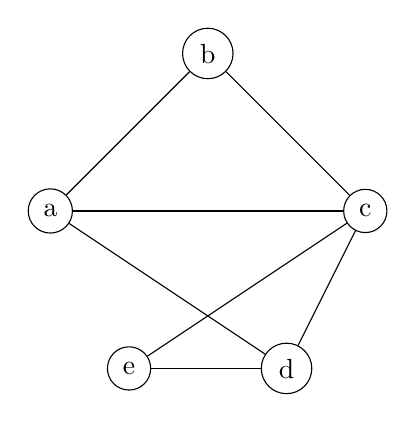
\begin{tikzpicture}[every node/.style={fill=white}, n/.style={circle, draw}]
			\node[n] (a) at (0, 0) {a};
			\node[n] (b) at (2, 2) {b};
			\node[n] (c) at (4, 0) {c};
			\node[n] (d) at (3, -2) {d};
			\node[n] (e) at (1, -2) {e};

			\draw (a) edge (b);
			\draw (a) edge (c);
			\draw (a) edge (d);
			\draw (b) edge (c);
			\draw (c) edge (d);
			\draw (c) edge (e);
			\draw (d) edge (e);
		\end{tikzpicture}

		\columnbreak

		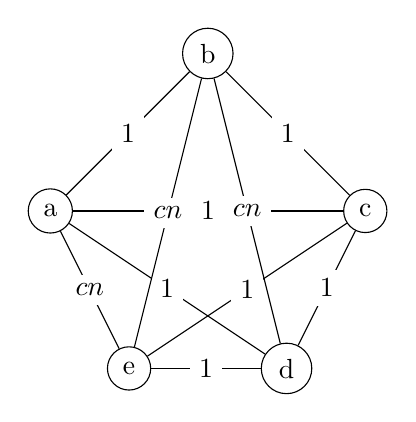
\begin{tikzpicture}[every node/.style={fill=white}, n/.style={circle, draw}]
			\node[n] (a) at (0, 0) {a};
			\node[n] (b) at (2, 2) {b};
			\node[n] (c) at (4, 0) {c};
			\node[n] (d) at (3, -2) {d};
			\node[n] (e) at (1, -2) {e};

			\draw (a) edge node {1} (b);
			\draw (a) edge node {1} (c);
			\draw (a) edge node {1} (d);
			\draw (b) edge node {1} (c);
			\draw (c) edge node {1} (d);
			\draw (c) edge node {1} (e);
			\draw (d) edge node {1} (e);
			\draw (a) edge node {$cn$} (e);
			\draw (b) edge node {$cn$} (d);
			\draw (b) edge node {$cn$} (e);
		\end{tikzpicture}
	\end{multicols}

	Se $G$ tem um circuito hamiltoniano, então $G'$ também tem um circuito hamiltoniano (o mesmo) de custo $n$ (porque as arestas têm peso 1). $\rightarrow \mathrm{OPT}(G', w)=n$

	Se $G$ não tem circuito hamiltoniano, então $G'$ tem (porque é completo), mas ele uma pelo menos uma aresta de custo $c \cdot n$. $\rightarrow \mathrm{OPT}(G', w) > c \cdot n$

	Relacionando com um algoritmo de aproximação: se existir um algoritmo $A$, que é uma $c$-aproximação para o TSP, então:

	Para o caso de $G$ ter um circuito hamiltoniano:
	\[
		A(G', w) \leq c \cdot \mathrm{OPT}(G', w) = c \cdot n
	\]

	Para o caso de $G$ \textbf{não} tiver um circuito hamiltoniano:
	\[
		A(G', w) \geq \mathrm{OPT(G', w)} > c \cdot n
	\]

	Sabemos então que, se o custo do algoritmo sobre $G'$ for menor ou igual a $c \cdot n$, sabemos que $G$ possui um circuito hamiltoniano (porque se o valor for maior, cai no segundo caso).

	Dessa forma, o algoritmo $A$ (de aproximação e polinomial) permitiria resolver o problema de decisão do Circuito Hamiltoniano, que é NP-Completo, então esse algoritmo não existe (a não ser que $P = NP$, aí existiria um algoritmo polinomial que resolva os problemas NP-Completos).
\end{example}


\subsection{TSP Métrico}

U grafo $G=(V, E)$ com peso $w$ nas arestas é métrico se ele for completo e se, para todo trio $u, v, x \in V$ temos que $w(uv) \leq w(ux) + w(xv)$ (desigualdade triangular). A ideia é a de que o caminho direto entre dois pontos seja mais barato que passando por outros pontos.

\begin{example}
	\begin{center}
		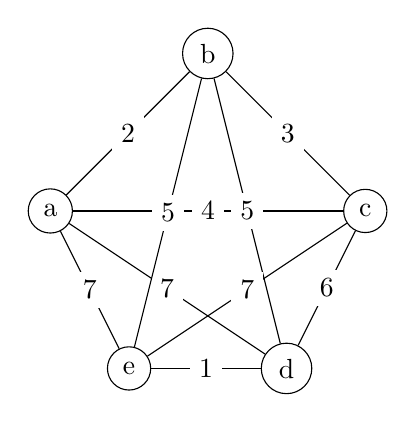
\begin{tikzpicture}[every node/.style={fill=white}, n/.style={circle, draw}]
			\node[n] (a) at (0, 0) {a};
			\node[n] (b) at (2, 2) {b};
			\node[n] (c) at (4, 0) {c};
			\node[n] (d) at (3, -2) {d};
			\node[n] (e) at (1, -2) {e};

			\draw (a) edge node {2} (b);
			\draw (a) edge node {4} (c);
			\draw (a) edge node {7} (d);
			\draw (a) edge node {7} (e);
			\draw (b) edge node {3} (c);
			\draw (b) edge node {5} (d);
			\draw (b) edge node {5} (e);
			\draw (c) edge node {6} (d);
			\draw (c) edge node {7} (e);
			\draw (d) edge node {1} (e);
		\end{tikzpicture}
	\end{center}
\end{example}

Um atalho é a troca de um caminho entre vértices $u$ e $v$, $(u, x_1, x_2, \dots, x_k, v)$, pela aresta $uv$. $\rightarrow$ A desigualdade triangular garante que o custo nunca aumenta com isso.

\begin{example}
	Primeiro, encontramos uma árvore geradora mínima (MST) $T$ de $G$ com custo $c(T)$.
	\begin{center}
		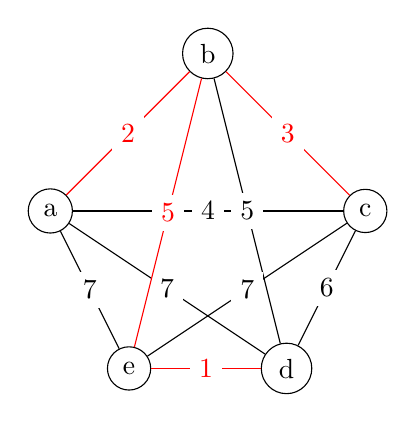
\begin{tikzpicture}[every node/.style={fill=white}, n/.style={circle, draw}]
			\node[n] (a) at (0, 0) {a};
			\node[n] (b) at (2, 2) {b};
			\node[n] (c) at (4, 0) {c};
			\node[n] (d) at (3, -2) {d};
			\node[n] (e) at (1, -2) {e};

			\draw[red] (a) edge node {2} (b);
			\draw (a) edge node {4} (c);
			\draw (a) edge node {7} (d);
			\draw (a) edge node {7} (e);
			\draw[red] (b) edge node {3} (c);
			\draw (b) edge node {5} (d);
			\draw[red] (b) edge node {5} (e);
			\draw (c) edge node {6} (d);
			\draw (c) edge node {7} (e);
			\draw[red] (d) edge node {1} (e);
		\end{tikzpicture}
	\end{center}

	Duplicamos as arestas de $T$. Esse grafo ($T^2$) tem custo $2c(T)$.

	\begin{center}
		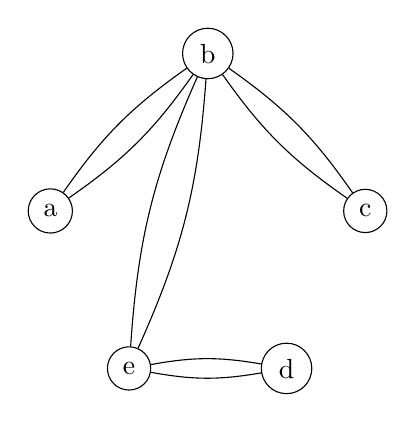
\begin{tikzpicture}[every node/.style={fill=white}, n/.style={circle, draw}]
			\node[n] (a) at (0, 0) {a};
			\node[n] (b) at (2, 2) {b};
			\node[n] (c) at (4, 0) {c};
			\node[n] (d) at (3, -2) {d};
			\node[n] (e) at (1, -2) {e};

			\draw[bend right=10] (a) edge (b);
			\draw[bend right=10] (b) edge (c);
			\draw[bend right=10] (b) edge (e);
			\draw[bend right=10] (d) edge (e);
			\draw[bend left=10] (a) edge (b);
			\draw[bend left=10] (b) edge (c);
			\draw[bend left=10] (b) edge (e);
			\draw[bend left=10] (d) edge (e);
		\end{tikzpicture}
	\end{center}

	Encontre um ciclo Euleriano $\varepsilon$ (percorre todas as arestas do grafo). Esse problema tem solução polinomial (o grau de todos os vértices tem que ser par). $c(\varepsilon) = c(T^2) = 2c(T)$.

	\begin{center}
		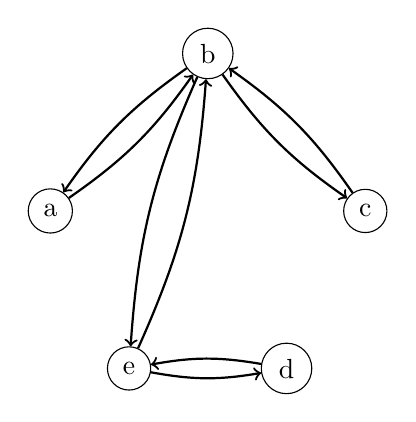
\begin{tikzpicture}[every node/.style={fill=white}, n/.style={circle, draw}]
			\node[n] (a) at (0, 0) {a};
			\node[n] (b) at (2, 2) {b};
			\node[n] (c) at (4, 0) {c};
			\node[n] (d) at (3, -2) {d};
			\node[n] (e) at (1, -2) {e};

			\draw[->, thick, bend right=10] (b) edge (a);
			\draw[->, thick, bend right=10] (c) edge (b);
			\draw[->, thick, bend right=10] (e) edge (b);
			\draw[->, thick, bend right=10] (e) edge (d);
			\draw[->, thick, bend right=10] (a) edge (b);
			\draw[->, thick, bend right=10] (b) edge (c);
			\draw[->, thick, bend right=10] (b) edge (e);
			\draw[->, thick, bend right=10] (d) edge (e);
		\end{tikzpicture}
	\end{center}

	\[
		\varepsilon = \left( a, b, c, b, e, d, e, b, a \right)
	\]

	Percorre $\varepsilon$ fazendo um atalho se for repetir um vértice.

	\begin{center}
		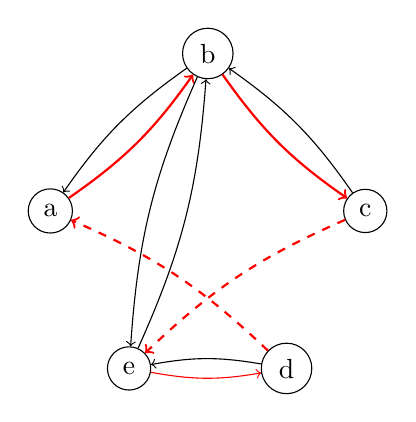
\begin{tikzpicture}[every node/.style={fill=white}, n/.style={circle, draw}]
			\node[n] (a) at (0, 0) {a};
			\node[n] (b) at (2, 2) {b};
			\node[n] (c) at (4, 0) {c};
			\node[n] (d) at (3, -2) {d};
			\node[n] (e) at (1, -2) {e};

			\draw[->, bend right=10] (b) edge (a);
			\draw[->, bend right=10] (c) edge (b);
			\draw[->, bend right=10] (e) edge (b);
			\draw[->, red, bend right=10] (e) edge (d);
			\draw[->, red, thick, bend right=10] (a) edge (b);
			\draw[->, red, thick, bend right=10] (b) edge (c);
			\draw[->, bend right=10] (b) edge (e);
			\draw[->, bend right=10] (d) edge (e);
			\draw[->, thick, red, dashed, bend right=10] (c) edge (e);
			\draw[->, thick, red, dashed, bend right=10] (d) edge (a);
		\end{tikzpicture}
	\end{center}

	\[
		\mathcal{C} = \left( a, b, c, e, d, a \right)
	\]

	Temos também a garantia de que $c(\mathcal{C}) \leq c(\varepsilon) = 2c(T)$. Isso só é garantido por causa da desigualdade triangular.

	\begin{align*}
		c(\mathcal{C}) & \leq c(\varepsilon)   \\
		               & = c(T^2)              \\
		               & = 2c(T)               \\
		               & \leq 2\mathrm{OPT}(I)
	\end{align*}

	Como $T$ é a árvore geradora \textbf{mínima}, seu custo é menor que o de qualquer árvore geradora. O seu custo também é menor que o custo de qualquer caminho que conecte todos os vértices de $G$ (já que é isso que uma MST faz). O custo da árvore também é menor que o de \underline{qualquer circuito} que visite todos os vértices de $G$ (porque o circuito vai ser um caminho, que já tem custo maior que a árvore, com mais uma aresta que volta pro início). Assim, o custo da árvore é inclusive menor que o da solução do TSP ($\mathrm{OPT}(I)$), que é um circuito de peso mínimo.
\end{example}

\subsection{Problema da Cobertura por Vértices}

\begin{itemize}
	\item \textbf{Entrada:} grafo $G=(V, E)$ com peso $w$ nas arestas.
	\item \textbf{Soluções viáveis:} subconjunto $S \subseteq V$ tal que para toda aresta $uv \in E$, $u \in S$ ou $v \in S$.
	\item \textbf{Função objetivo:} soma dos pesos dos vértices em $S$.
	\item \textbf{Objetivo:} encontrar solução de custo mínimo.
\end{itemize}

É um caso particular da \hyperref[sec:cobertura_conjuntos]{Cobertura por Conjuntos} (\hyperref[chp:semana4]{Semana 4}). Então é possível reduzir esse problema para o de \hyperref[sec:cobertura_conjuntos]{Cobertura por Conjuntos}.

\begin{example}
	\begin{center}
		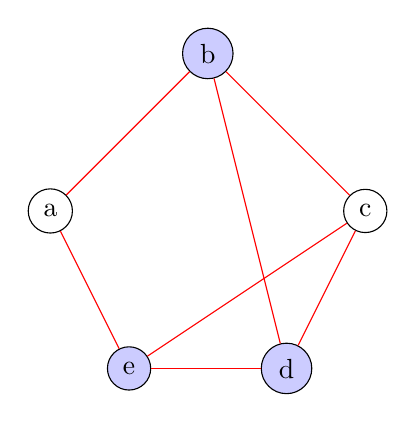
\begin{tikzpicture}[every node/.style={fill=white}, n/.style={circle, draw}]
			\node[n] (a) at (0, 0) {a};
			\node[n, fill=blue!20] (b) at (2, 2) {b};
			\node[n] (c) at (4, 0) {c};
			\node[n, fill=blue!20] (d) at (3, -2) {d};
			\node[n, fill=blue!20] (e) at (1, -2) {e};

			\draw[red] (a) edge (b);
			\draw[red] (a) edge (e);
			\draw[red] (b) edge (c);
			\draw[red] (b) edge (d);
			\draw[red] (c) edge (d);
			\draw[red] (c) edge (e);
			\draw[red] (d) edge (e);
		\end{tikzpicture}
	\end{center}
\end{example}

Começamos com a formulação do problema em PLI.

\begin{itemize}
	\item Variáveis: $x_v \quad \forall v \in V$. Indica se o vértice $v$ foi escolhido.
	\item Função objetivo: $\min\sum_{v \in V}w_vx_v$. Minimizar o custo dos nós escolhidos.
	\item Restrição: $x_u + x_v \geq 1 \quad \forall uv \in E$. Para toda aresta, pelo menos uma ponta tem que estar na solução.
	\item Domínio das variáveis: $x_v \in \left\{ 0, 1\right\} \quad \forall v \in V$.
\end{itemize}

Programação Linear (não a interira) pode ser utilizada para encontrar soluções aproximadas (a partir da relaxação de integralidade do problema). E a solução desse PL é um \textbf{limitante inferior} da solução do problema.

\begin{algorithm}
	\SetAlgoLined
	\SetKwFunction{VertexCoverAprox}{VertexCoverAprox}
	\Fn{\VertexCoverAprox{$G=(V, E), w$}}{
		Monte e resolva o PL, obtendo $x^*$\;
		\tcc{Fazemos um arredondamento determinístico do resultado do PL}
		\Para{$v \in V$}{
			\lSe{$x_v^* \geq 1$}{$x_v \gets 1$}
			\lSenao{$x_v \gets 0$}
		}
		\Retorna{$\sum_{v \in V}w_vx_v$}
	}
\end{algorithm}

A solução é viável, porque, como toda aresta satisfaz $x_u^* + x_v^* \geq 1$, pelo menos $x_u^*$ ou $x_v^*$ tem que ser maior 0,5 (senão a soma nunca chega em 1). Assim, pelo menos uma das variáveis em cada restrição vai ser arredondada para 1 $\rightarrow$ Garante a viabilidade da solução inteira aproximada.

Como esse algoritmo faz o arredondamento determinístico, também é possível aleatorizar.

Com relação ao custo da solução, temos alguns casos específicos:

\begin{itemize}
	\item Se $x_v = 1$, então $x_v^* \geq 0,5 \rightarrow x_v = 1 \leq 2x_v^*$.
	\item Se $x_v = 0$, então também vale que $x_v = 0 \leq 2x_v^*$.
\end{itemize}

\begin{align*}
	\text{\lstinline{VertexCoverAprox}}(I) & = \sum_{v \in V}w_vx_v\\
	  & \leq \sum_{v \in V}w_v(2x_v^*)    \\
	  & = 2 \sum_{v \in V}  w_vx_v^*      \\
	  & = 2 \mathrm{OPT}_{\mathrm{PL}}(I) \\
	  & \leq 2\mathrm{OPT}(I)
\end{align*}

O algoritmo é uma 2-aproximação.

É possível generalizar o algoritmo para tratar o problema da \hyperref[sec:cobertura_conjuntos]{Cobertura por Conjuntos}. Isso depende da maneira de fazer a redução do problema e adaptação da razão para fazer o arredondamento.

\section{Parametrização}

Esse é um exemplo de abordagem em que relaxamos a restrição de resolver \textbf{qualquer} instância.

Uma abordagem mais recente é a de Complexidade Parametrizada. Queremos analisar as características do problema para identificar qual é o parâmetro ($k$) que influencia na complexidade dos algoritmos usados, ainda que a instância seja grande, se controlar o $k$ podemos conseguir a solução em tempo hábil.

\begin{quote}
	``Dada uma entrada $I$ e um inteiro não negativo $k$, $I$ tem alguma propriedade que depende de $k$?''
\end{quote}

Queremos encontrar algoritmos que são exponenciais apenas com relação a $k$ e polinomiais com relação ao tamanho $n$ de $I$. $\rightarrow O(n^cf(k))$

Problemas desse tipo pertencem à classe FPT (\textit{Fixed-Parameter Tractable}), tratáveis caso o parâmetro seja fixo.

\subsection{Problema da k Cobertura por Vértices}

\begin{itemize}
	\item \textbf{Entrada:} grafo $G=(V, E)$ e inteiro positivo $k$.
	\item \textbf{Questão:} $G$ possui uma solução $S$ tal que $|S| \leq k$ e, para toda aresta $uv \in E$, $u \in S$ ou $v \in S$?
\end{itemize}

Só estamos interessados se a cobertura for pequena (estipulado por $k$), mesmo se o grafo for grande (com muitos vértices).

\begin{example}
	\centering
	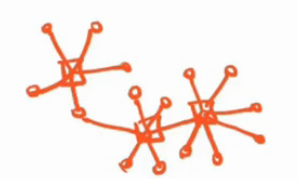
\includegraphics[scale=.75]{img/ex_k_cobertura_pequena.png}
\end{example}

\begin{algorithm}
	\SetAlgoLined
	\SetKwFunction{VertexCoverK}{VertexCoverK}
	\Fn{\VertexCoverK{$G=(V, E), k$}}{
		\Se{$G$ não possui arestas}{
			\Retorna{SIM}
		}
		\Se{$k = 0$}{
			\Retorna{NÃO}
		}
		Escolha uma aresta $uv$ arbitrariamente\;
		\tcc{Pelo pelo um dos extremos tem que estar na cobertura}
		\Se{\VertexCoverK{$G-u, k-1$} retornar SIM}{
			\tcc{Existe uma cobertura do resto do grafo (já removemos o $u$ e todas as arestas cobertas por ele) que usa $k-1$ vértices (já que $u$ já foi usado para cobrir)?}
			\Retorna{SIM}
		}
		\Se{\VertexCoverK{$G-v, k-1$} retornar SIM}{
			\tcc{$u$ não funcionou para cobrir o grafo, mas podemos tentar fazendo a cobertura pelo vértice $v$}
			\Retorna{SIM}
		}
		\Retorna{NAO} \tcc*{Não conseguimos $k$ vértices que cubram o grafo}
	}
\end{algorithm}

A complexidade do algoritmo é $O(|V|\cdot 2^k)$: no pior caso, efetua duas chamadas recursivas (para o $u$ e para o $v$), mas a árvore de busca tem altura de, no máximo, $k$. O algoritmo é exponencial, mas a questão é que \textbf{para $\mathbf{k}$ pequeno} (no máximo $\log |V|$), o crescimento exponencial está controlado.
